\chapter{StaMPS Persistent Scatterer Interferometry}

\begin{figure}[H]
\centering
\includegraphics[width=0.8\columnwidth]{images/PHASE_mod1b.png}
\end{figure}

\section{Open a prepared dataset}
After preprocessing, select \textbf{StaMPS PSI} in the same PHASE window. Choose the dataset from the selector at the top of the module; \textbf{Refresh} rescans the project's prepared datasets. The working directory is shown below it. The shared StaMPS and, when needed, TRAIN runtimes are installed with PHASE and remain outside the project folder. Do not move the applications or copy the runtime into individual projects.

Windows and macOS Apple Silicon have been exercised with end-to-end PSI runs. Linux is distributed with an experimental native build path, but a complete PSI run has not yet been independently validated there. Always review the current release notes and prerequisites before relying on a result.

\section{Configure the analysis}
The sidebar contains \textbf{Project}, \textbf{Global variables}, \textbf{Steps 1--8}, \textbf{Export}, \textbf{Run monitor} and \textbf{TS Points}. \textbf{Show all parameters} is enabled by default; hide advanced controls if you prefer a shorter view. Set the first and last StaMPS steps deliberately: the first full run normally includes data preparation and the steps needed for phase-noise estimation, PS selection, weeding, unwrapping, spatially correlated look-angle error estimation, and optional Step 8 filtering. A partial rerun depends on the preceding intermediate products.

\begin{figure}[htbp]
\centering
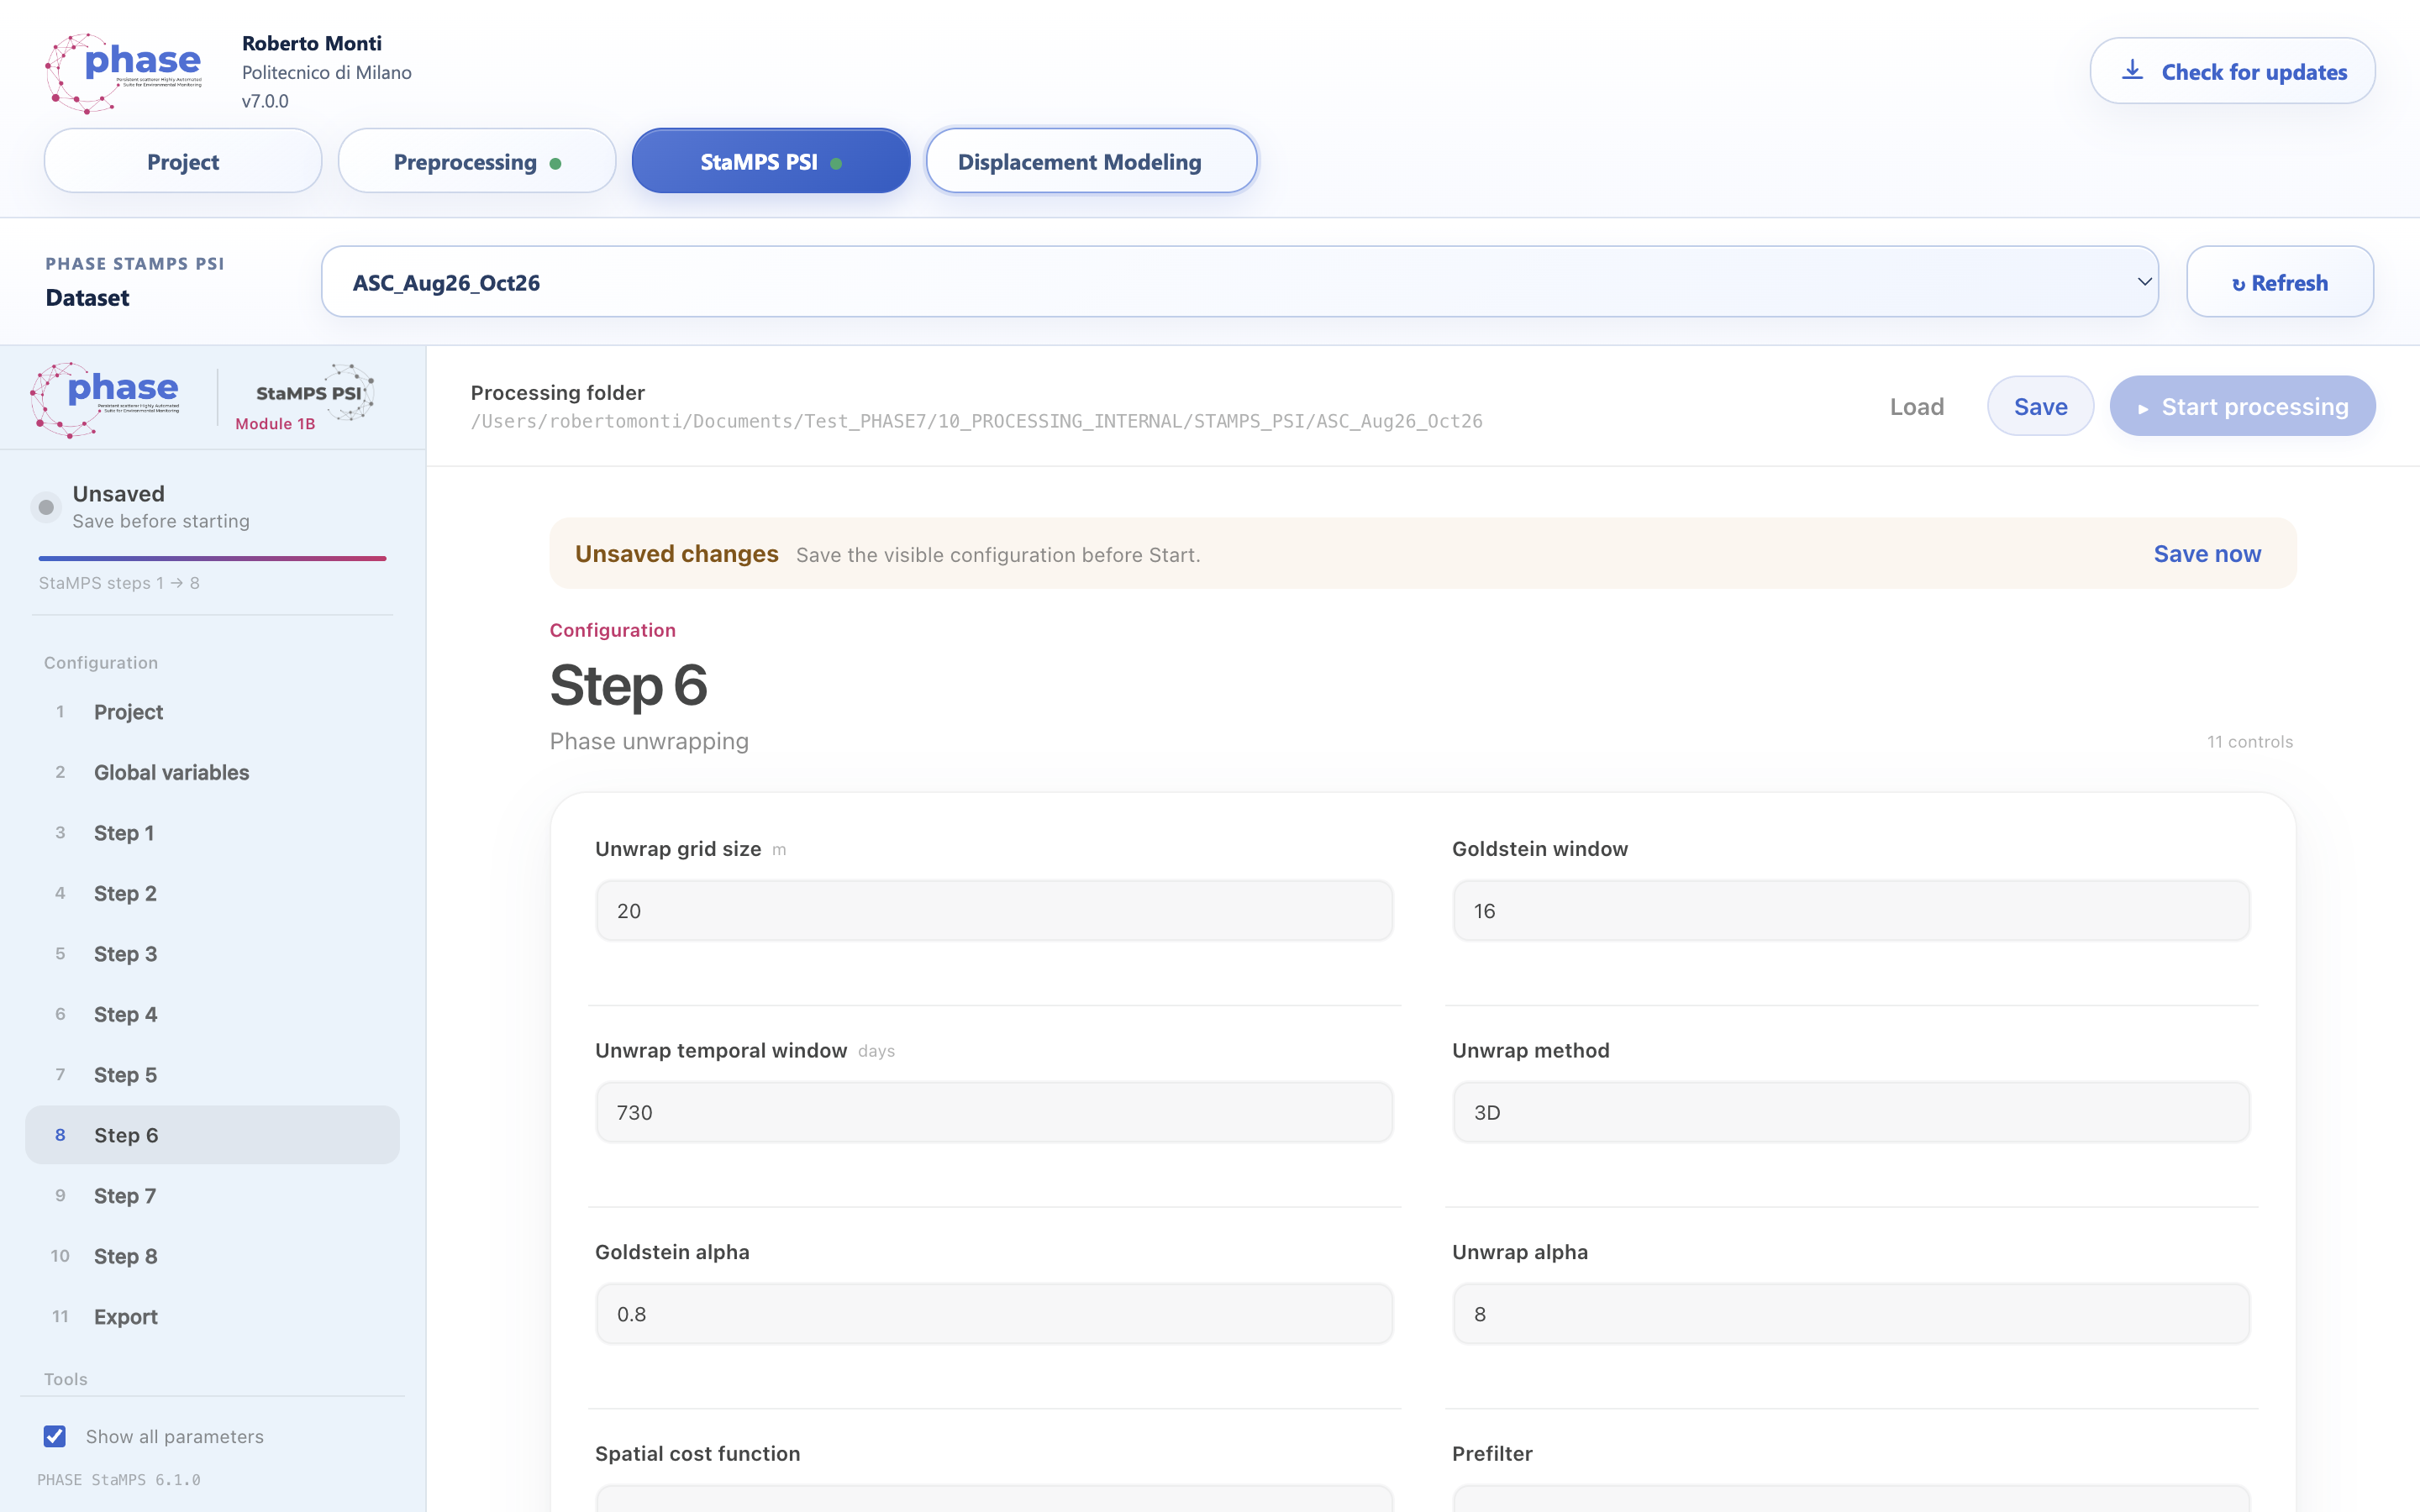
\includegraphics[width=\textwidth]{images/Screenshot 2026-10-11 alle 23.11.13.png}
\caption{StaMPS PSI within the unified hub. This example shows the Step 6 phase-unwrapping controls; the numerical values belong to the test project and should not be copied without analysis.}
\label{fig:phase7-stamps}
\end{figure}

PHASE detects key metadata where possible, including the master date and acquisition parameters. Inspect the automatically filled values against the source stack, especially after importing data from another processing system. The amplitude-dispersion threshold and phase-noise criteria control candidate density; relaxing them may increase the number of points while also adding noisy scatterers. Select a stable reference area or point appropriate for the study, because displacement is relative to a reference in space and time.

\subsection{Key StaMPS stages}
\begin{description}[style=nextline]
\item[Step 1 --- data preparation] Convert SNAP/StaMPS inputs and organize the interferogram stack.
\item[Steps 2--4 --- estimation and selection] Estimate phase noise, select PS candidates and remove inconsistent points.
\item[Steps 5--6 --- correction and unwrapping] Prepare corrected phase and unwrap it in space and time.
\item[Step 7 --- SCLA and ramp] Estimate spatially correlated look-angle/DEM error and, if configured, an orbital ramp.
\item[Step 8 --- spatially correlated noise] Optionally filter residual spatially correlated noise. Atmospheric delay can be a major component, but the Step 8 estimate is not guaranteed to be purely atmospheric and can absorb real spatially correlated deformation.
\end{description}

Consult the StaMPS manual for the scientific definition and interaction of individual parameters. PHASE presents them in a GUI but does not change their interpretation.

\section{Atmospheric correction and export choice}\label{ss:tropo}
PHASE offers an explicit \textbf{Standard} or \textbf{Corrected} displacement export. The choice controls both the automatic full CSV/XLSX series and the optional TS Points export. It is not inferred from whether the processing reached Step 8.

\begin{table}[htbp]
\centering
\caption{Displacement series exported through StaMPS \texttt{ps\_plot}.}
\begin{tabular}{@{}p{2.4cm}p{4.2cm}p{1.6cm}p{4.2cm}@{}}
\toprule
\textbf{Choice} & \textbf{Available source} & \textbf{Type} & \textbf{Additional subtraction at export} \\
\midrule
Standard & Step 7 or Step 8 & \texttt{v-do} & No additional \texttt{a} or \texttt{s} term \\
Corrected & TRAIN estimate available & \texttt{v-dao} & TRAIN tropospheric estimate, plus \texttt{d} and \texttt{o} \\
Corrected & No TRAIN; Step 8 completed & \texttt{v-dso} & Step 8 spatially correlated noise, plus \texttt{d} and \texttt{o} \\
\bottomrule
\end{tabular}
\end{table}

Here \texttt{d} denotes SCLA/DEM error and \texttt{o} an orbital ramp. Standard \texttt{v-do} means no \emph{additional} atmospheric subtraction in the export operation; it does not prove that no atmospheric effect was treated upstream. Corrected \texttt{v-dso} should be described as Step 8 spatial-noise-corrected, not as a pure atmospheric correction. If both TRAIN and Step 8 are configured, PHASE uses \texttt{v-dao} for the corrected export and does not silently combine the two estimates. If the requested TRAIN correction is unavailable, the corrected export fails rather than silently reverting to Standard.

TRAIN can be configured with a linear phase--topography model (\texttt{a\_linear}) or, when appropriate data are available, GACOS (\texttt{a\_gacos}). GACOS requires externally supplied atmospheric products and may pause the workflow while they are obtained; follow the paths and instructions displayed by the running application rather than an old, hard-coded folder example. Validate availability, date coverage and units before resuming. Correction can remove a geophysical component along with noise, so compare Standard and Corrected series when interpreting broad spatial signals.

\section{Run monitor and outputs}
Save the configuration and choose \textbf{Start processing}. The \textbf{Run monitor} displays the selected step range, correction and export summary, the current operation, a progress estimate, elapsed time and the processing log. Progress is based on StaMPS steps and patches; it is not proportional to elapsed time. Keep the run/error log for reproducibility, especially if native binaries or MATLAB stop unexpectedly.

PHASE automatically exports the complete point time series to CSV and XLSX. Displacements are in millimetres and velocity is in millimetres per year. The master epoch is the temporal zero; PHASE inserts a zero-valued master epoch only when it is absent from the StaMPS time axis. Export metadata record the chosen StaMPS value type in a \texttt{\_series.json} file. Inspect that metadata before comparing results produced with different correction modes. The exports are placed in the project's results area, while detailed processing files and logs remain separated.

The \textbf{TS Points} section and the \textbf{Explore TS Points} action in the Run monitor provide an \emph{optional} point-by-point inspection and selected-point export. They are not necessary to obtain the complete series. The picker is integrated into the StaMPS section and can be opened later from an already completed unwrapped PSI dataset. It uses the same export mode as the full series.

\begin{figure}[htbp]
\centering
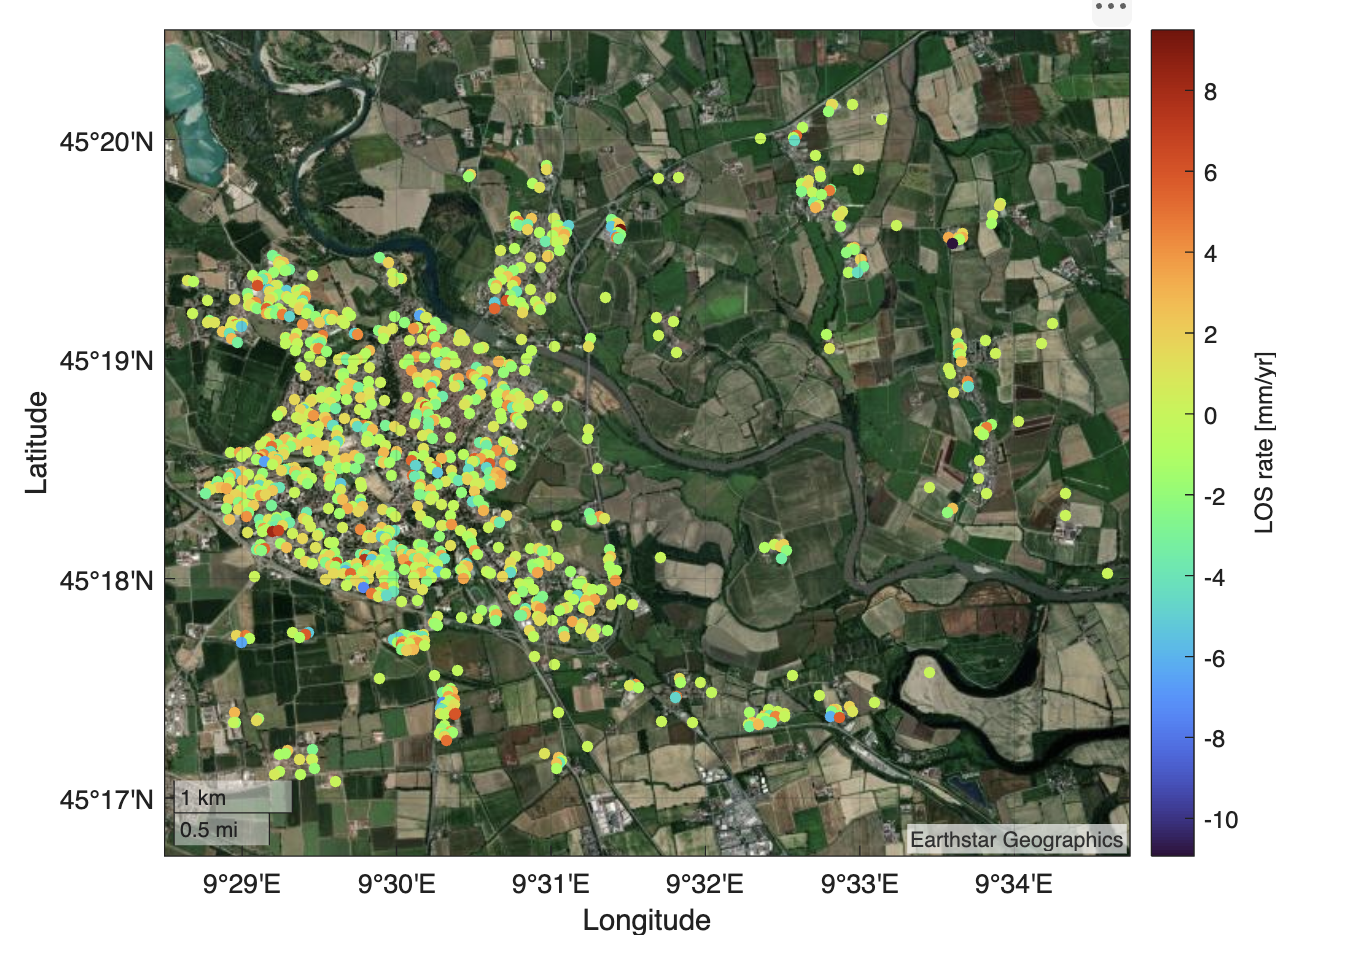
\includegraphics[width=0.9\textwidth]{images/PHASE_v7_PSI_output_example.png}
\caption{Example LOS velocity visualization from a PHASE 7 macOS PSI run. This operational test image does not independently validate the deformation estimates or establish the export correction mode.}
\end{figure}

\section{Quality checks and troubleshooting}
Before modeling, inspect the spatial distribution of PS points, temporal coverage, coherence/phase quality, the reference area and the sign and scale of LOS rates. Investigate large jumps, isolated outliers and differences between Standard and Corrected series; a visually plausible map alone is insufficient validation. Compare with independent measurements where available.

\begin{description}[style=nextline]
\item[No prepared dataset] Return to Preprocessing and check that StaMPS inputs were exported successfully; then use \textbf{Refresh}.
\item[Step 1 native-tool or Python error] Save the complete run log and verify that the installed PHASE runtime and prerequisites are accessible. Avoid modifying the shared runtime or project data without identifying the failing command.
\item[Correction unavailable] Confirm the selected TRAIN/GACOS inputs or complete Step 8 if using its correction. Do not interpret a Standard fallback as a corrected series.
\item[Unexpected point count] Revisit amplitude-dispersion and PS-selection settings, but avoid increasing density without checking noise and unwrapping quality.
\end{description}
